\documentclass[./dokumentation.tex]{subfiles}

\begin{document}
\chapter{Emotionen - Grundlagen}
Nach  \cite{vanGorp2013} können Emotionen anhand von zwei grundlegenden Dimensionen beschrieben werden. Diese Dimensionen sind Wert (Value) und Erregung (Arousal). Den Wert von etwas bestimmen wir irgendwo zwischen Gut und Böse, was häufig mit angenehm oder unangenehm verknüpft wird. \\
Bei Erregung handelt es sich um die unbewusste Aktivierung des Körpers, Gehirns oder eines bestimmten Verhaltens. Dieses wird durch das Ausmaß von Angst gegenüber Schläfrigkeit definiert und kann beispielsweise durch das Überwachen von Herzfrequenz, Atmung oder Blutdruck gemessen werden. Werden beide Emotionsdimensionen, also das Bewusste, Kognitive und das Unbewusste, Körperliche kombiniert, erhält man das kreisförmige Emotionsmodell, welches in ähnlicher Form schon 1980 von Russell aufgestellt wurde.\\ 
Dieses ist in der folgenden Darstellung (\ref{fig4:affect}) abgebildet und enthält noch zusätzlich Affekte, wie Zufriedenheit (Contentment), Aufregung (Excitement), Not, Verzweiflung (Distress) und Niedergeschlagenheit (Depression), welche jeweils zwischen den Achsen eingeordnet werden können  \cite{Russell1980}. \\

\begin{figure}[H]
    \centering
    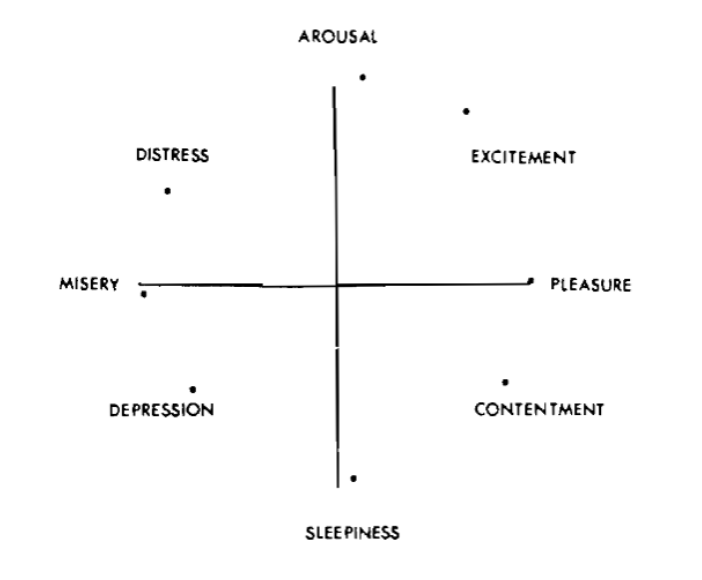
\includegraphics[width=0.8\textwidth]{bilder/russell1.png}
    \caption{Acht Affektkonzepte in kreisförmiger Ordnung \cite{Russell1980}}
    \label{fig4:affect}
\end{figure}\\

Analog dazu können auch weitere Affekte in den Kreis eingeordnet werden. In der folgenden Abbildung (\ref{fig5:28affect}) nach Russell sind 28 Affekte innerhalb des Kreises dargestellt.

\begin{figure}[H]
    \centering
    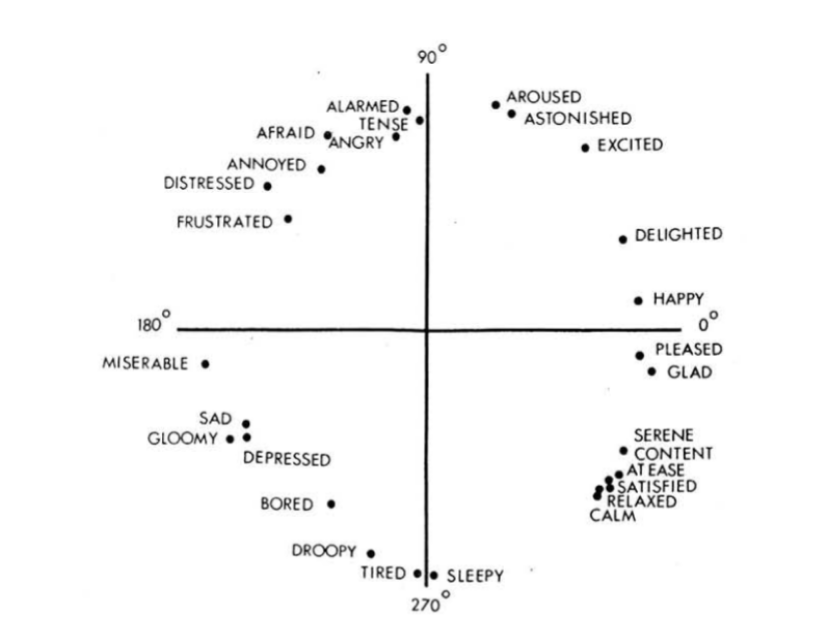
\includegraphics[width=0.8\textwidth]{bilder/russell2.png}
    \caption{Direkte kreisförmige Skalierungskoordinaten für 28 Affektwörter \cite{Russell1980}}
    \label{fig5:28affect}
\end{figure}\\

\section{Gelassenheit}
,,Gelassenheit'' ist eine emotionale Zustandsform, die eng mit innerer Ruhe, Entspannung und Ausgeglichenheit verbunden ist. Es ist eine positive Emotion, die oft als das Gegenteil von Stress, Angst und Anspannung betrachtet wird. Menschen, die gelassen sind, fühlen sich in der Regel ruhig, gelöst und frei von Stress. \\
Die Emotion der Gelassenheit entsteht, wenn eine Person in der Lage ist, sich von äußeren Unruhefaktoren und Herausforderungen nicht übermäßig beeinflussen zu lassen. Es geht darum, contenance und in schwierigen Situationen eine innere Stabilität zu bewahren. Gelassenheit beinhaltet auch das Bewusstsein für die eigenen Gefühle und Gedanken sowie die Fähigkeit, sie auf eine positive und konstruktive Weise zu regulieren. \\
Menschen, die gelassen sind, können oft besser mit Stress und Herausforderungen umgehen, da sie nicht von ihnen überwältigt werden. Sie sind in der Lage, klarer zu denken und angemessen zu handeln, selbst in schwierigen Situationen. Die Gelassenheit ermöglicht es einer Person, sich auf das Hier und Jetzt zu konzentrieren.\\

Gelassenheit ist keine Emotion, die man einfach ,,hat'' oder ,,nicht hat''. Es ist vielmehr eine Fähigkeit, die entwickelt und kultiviert werden kann. Meditation, Achtsamkeitsübungen und Entspannungstechniken sind einige der Methoden, die Menschen dabei unterstützen können, innere Gelassenheit zu erlangen. Gelassenheit bedeutet nicht, dass man niemals negativen Gefühlen ausgesetzt ist. Stattdessen geht es darum, sie auf eine gesunde Weise zu verarbeiten und ihnen nicht die Kontrolle über das eigene Leben zu überlassen. \\
Die Gelassenheit kann viele positive Auswirkungen auf das körperliche und geistige Wohlbefinden haben. Studien haben gezeigt, dass gelassene Menschen oft ein niedrigeres Stressniveau haben, was sich positiv auf das Herz-Kreislauf-System und das Immunsystem auswirken kann \cite{chin2021}. Darüber hinaus kann Gelassenheit auch zu einer besseren Bewältigung von Angststörungen, Depressionen und anderen psychischen Herausforderungen beitragen \cite{monahan1986}. \\
In der heutigen hektischen und schnelllebigen urbanen Welt ist die Fähigkeit, Gelassenheit zu erlangen, eine sinnvolle Methode der Stressbewältigung. Dazu kann es sinnvoll sein, sich bewusst einer natürlichen Umgebung auszusetzen \cite{vandenbosch2015}. Eine gelassene Haltung kann dazu beitragen, dass man sich weniger gestresst oder hektisch fühlt und bessere, bewusstere Entscheidungen trifft. \\
In Bezug auf das gestalterische Thema der Webseite, die Gelassenheit erzeugen soll, spielt die Auswahl von Farben und Kontrasten eine entscheidende Rolle, um diese emotionale Zustandsform zu unterstützen. Dabei sollen darüber hinaus ablenkende auditive und visuelle Reize vermieden werden. Die bewusste Verwendung von sanften Farben wie Grüntönen, angelehnt an die Natur, und geringen Kontrasten kann dazu beitragen, dass die Besucher der Webseite eine ruhigere und entspannte Atmosphäre wahrnehmen, was wiederum ihre Gelassenheit und Wohlbefinden positiv beeinflussen kann.

\section{Nostalgie}

\section{Stress - Unsicherheit}
\end{document}


